%
% File: chap01.tex
% Author: Victor F. Brena-Medina
% Description: Introduction chapter where the biology goes.
%
\let\textcircled=\pgftextcircled
\chapter{Introduction}
\label{chap:intro}

\initial{B}egins a chapter. Example: When the beloved cellist (Christopher Walken - outstanding) of a world-renowned string quartet receives a life-changing diagnosis, the group's future suddenly hangs in the balance: suppressed emotions, competing egos and uncontrollable passions threaten to derail years of friendship and collaboration. Featuring a brilliant ensemble cast (including Philip Seymour Hoffman, Catherine Keener and Mark Ivanir as the three other quartet members), it is a fascinating look into the world of working musicians, and an elegant homage to chamber music and the cultural world of New York. The music, of course, is ravishing (the score is the work of regular David Lynch collaborator Angelo Badalamenti): A Late Quartet hits all the right notes.

%=======
\section{Section}
\label{sec:sec01}

Begins a section.

\subsection{Subsection}
\label{subsec:subsec01}

Begins a subsection.

%A figures matrix.
\begin{figure}[t!]
\centering
\begin{minipage}{3.3cm}
    \centering
    \subtop[]{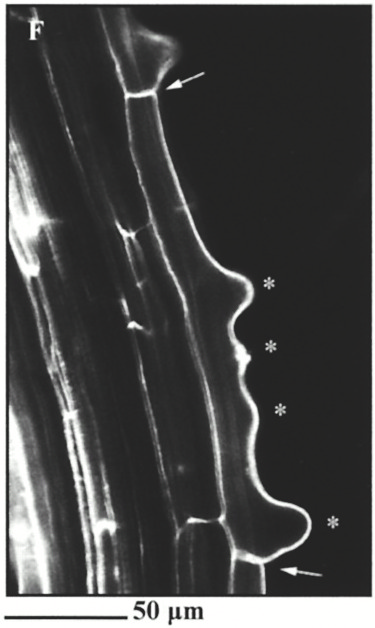
\includegraphics[height=0.28\textheight]{fig01/Nswellings}\label{sf:multiRH02a}}
\end{minipage}
\hspace{0.5cm}
\begin{minipage}{3.3cm}
    \centering
    \subtop[]{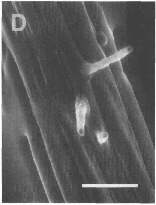
\includegraphics[height=0.27\textheight]{fig01/Mswellings}\label{sf:multiRH02b}}
\end{minipage}
\hspace{1.3cm}
\begin{minipage}{3.3cm}
    \centering
    \subtop[]{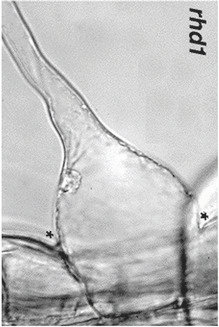
\includegraphics[height=0.27\textheight]{fig01/rhd1}\label{sf:multiRH02c}}
\end{minipage}
\\ \vspace{0.1cm}
\begin{minipage}{10cm}
    \centering
    \subtop[]{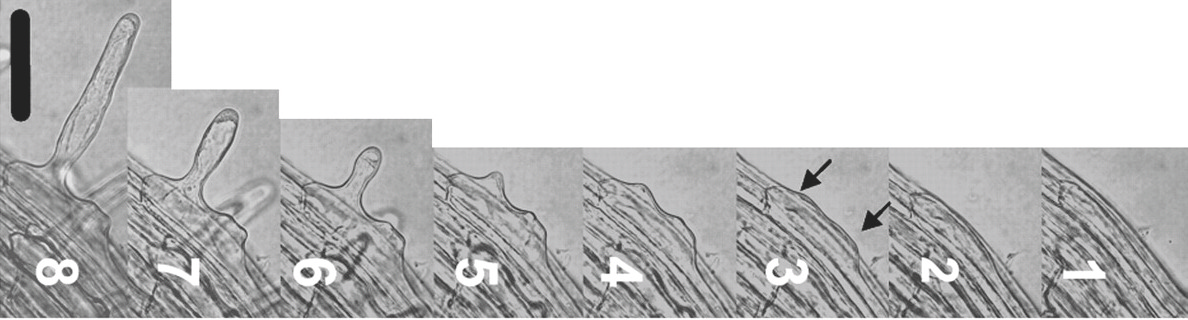
\includegraphics[height=0.145\textheight]{fig01/mutantrhd6}\label{sf:multiRH02d}}
\end{minipage}
\\ \vspace{0.1cm}
\begin{minipage}{10cm}
    \centering
    \subtop[]{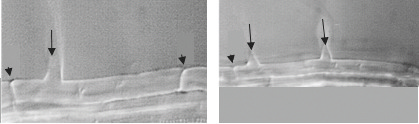
\includegraphics[height=0.16\textheight]{fig01/auxab}\label{sf:multiRH02e}}
\end{minipage}
\mycaption[Hair-forming mutant cells.]{(a) A mutant RH cell. Asterisks show multiple sites of RH initiation in a single root hair cell (indicated by the arrows). Figure reproduced from \cite{rigas01}. (b)~Hair-forming cell with three RH initiation locations. The bar represents $50\mu m$. Figure reproduced from \cite{massuci01}. (c) Large bump in mutant {\itshape rhd1}. Figure reproduced from \cite{griersonRH}. (d) Mutant overexpressing gene {\itshape ROP2}; from right-hand to left-hand, numbers indicate progressive snapshots at different times. RH initiation sites are indicated by the arrows. The bar represents $75\mu m$. Figure reproduced from~\cite{mjones01}. (e)~Mutants affected by auxin. On the left-hand side, RH site is farther away from the apical end (left arrow cap); on the right-hand side, multiple RH locations (arrows). Figure reproduced from~\cite{payne01}.}
\label{fig:multiRH02}
\end{figure}

% A single figure
\begin{figure}[t!]
	\centering
	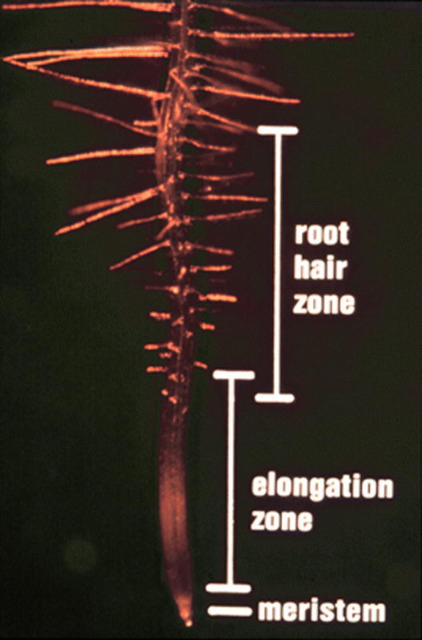
\includegraphics[height=0.35\textheight]{fig01/devepzones}
	\mycaption[Developmental zones of an Arabidopsis root.]{Developmental zones of an Arabidopsis root. Figure reproduced from \cite{griersonRH}.}
	\label{fig:RHP02}
\end{figure}

%=========================================================